\documentclass[journal]{IEEEtran}

\usepackage[T1]{fontenc}
\usepackage[utf8]{inputenc}
\usepackage{amsmath,amssymb,amsfonts}
\usepackage{graphicx}
\usepackage{booktabs}
\usepackage{array}
\usepackage{url}
\usepackage{xcolor}
\usepackage[hidelinks]{hyperref}
\usepackage{orcidlink}
\usepackage{balance}

\graphicspath{{../figures/}}

\renewcommand{\topfraction}{0.92}
\renewcommand{\bottomfraction}{0.75}
\renewcommand{\textfraction}{0.08}
\renewcommand{\floatpagefraction}{0.80}

\begin{document}

\title{TailWatch: An InSAR Deformation-Monitoring and\\ Inverse-Velocity Failure-Forecasting Studio,\\ on Synthetic Sentinel-1 and Real Campi Flegrei}

\author{Felipe~Santiba\~nez-Leal~\orcidlink{0000-0002-0150-3246}%
\thanks{F. Santiba\~nez-Leal is with the CAOS open-research programme, Santiago, Chile
(e-mail: fsantibanez@gmail.com; ORCID 0000-0002-0150-3246).}%
\thanks{Technical report, 2026. Interactive studio and reproducible pipeline (MIT) at
\url{https://github.com/fsantibanezleal/CAOS_TailWatch}; live at \url{https://tailwatch.fasl-work.com}.}}

\markboth{Technical Report, 2026}%
{Santiba\~nez-Leal: An InSAR deformation-monitoring and failure-forecasting studio}

\maketitle

\begin{abstract}
Ground deformation is the earliest measurable warning of a tailings-dam or pit-wall failure, and satellite
interferometric synthetic-aperture radar (InSAR) can measure it at the millimetre scale over a whole facility.
This report describes TailWatch, an interactive, reproducible studio that carries a deformation field from
InSAR displacement to a failure forecast, and reports the honest accuracy of each stage. Two data lanes feed it:
a high-fidelity synthetic Sentinel-1 forward simulation (von-K\'arm\'an atmospheric phase screen, decorrelation,
digital-elevation-model error and orbital ramps) over five deformation regimes, and one \emph{real} case, the
Campi Flegrei caldera from the open COMET LiCSAR/LiCSBAS Sentinel-1 archive. A two-geometry Up/East decomposition
resolves the line-of-sight field; a learned tier flags anomalies and classifies deformation type; and a classical
inverse-velocity model forecasts the time of failure. The results are measured and honest. The anomaly detectors
are strong (velocity-based area-under-curve $0.968$, autoencoder $0.898$), and while the six-class
deformation-type classifier is only moderate overall (macro-F1 $0.556$), it recovers the one class that matters
for early warning, \emph{accelerating}, at $0.99$ recall. The inverse-velocity forecast detects every
accelerating failure ($100\%$) with a median failure-time error of $3.8\%$ on synthetic cases and $5.7\%$ on the
real Campi Flegrei data, tightening from about $14\%$ far ahead to $2\%$ close to failure, exactly the behaviour a
warning system needs. We are explicit that this is a didactic and decision-support instrument, not a certified
safety system, that most cases are synthetic with one real anchor, and that the small-baseline network inversion
is on the roadmap; every number and figure regenerates from the committed artifacts.
\end{abstract}

\begin{IEEEkeywords}
InSAR, ground deformation, tailings dam, slope stability, inverse velocity, failure forecasting, anomaly
detection, Sentinel-1, Campi Flegrei, reproducibility.
\end{IEEEkeywords}

\section{Introduction}

\IEEEPARstart{T}{he} failure of a tailings storage facility or a pit wall is preceded, often by weeks, by
accelerating ground deformation, and measuring that deformation early is the core of geotechnical risk
management. Satellite interferometric synthetic-aperture radar (InSAR) is uniquely suited to it: by comparing the
phase of radar returns across repeated passes it measures line-of-sight displacement at the millimetre scale over
an entire facility, without instrumenting the ground~\cite{massonnet,rosen}. Two families of processing make the
measurement robust to noise, persistent-scatterer interferometry~\cite{ferretti} and small-baseline subset
(SBAS) time-series analysis~\cite{berardino,hooper}, and the open Sentinel-1 archive, processed by automated
pipelines such as LiCSAR and LiCSBAS~\cite{lazecky,morishita}, has made global monitoring routine. What a mine
operator needs from that displacement field is not the field itself but a decision: is anything anomalous, what
kind of movement is it, and, if it is accelerating, when will it fail?

TailWatch is an interactive studio that makes that chain explicit and honest, and this report describes it and
measures each stage. It is built on two data lanes (Fig.~\ref{fig:arch}). The first is a high-fidelity synthetic
Sentinel-1 forward simulation, which lets the pipeline be exercised over controlled deformation regimes with
known ground truth; the second is a single \emph{real} case, the Campi Flegrei caldera near Pozzuoli, drawn from
the open COMET LiCSAR/LiCSBAS Sentinel-1 archive, which anchors the forecast on genuine data. From the
displacement field a two-geometry decomposition resolves vertical and east-west motion, a learned tier flags
spatial anomalies and classifies each pixel's deformation type, and a classical inverse-velocity model projects
the failure time with a tiered alarm. The contribution is not a new InSAR algorithm; it is a reproducible,
end-to-end studio with the honest accuracy of each stage reported, including where it is strong and where it is
only moderate.

\section{The Pipeline and Its Data}\label{sec:pipeline}

\begin{figure}[!t]
\centering
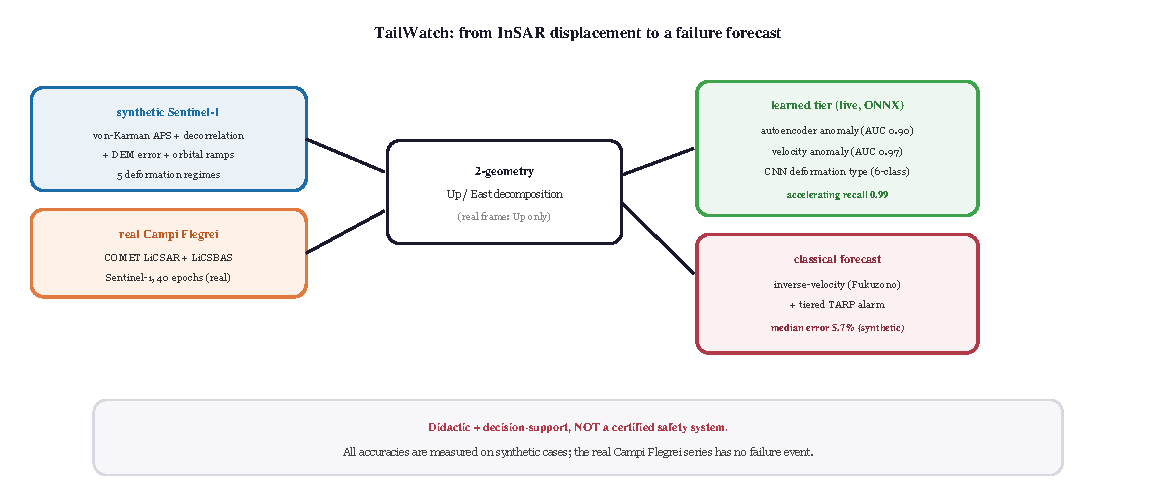
\includegraphics[width=0.99\columnwidth]{fig-arch.pdf}
\caption{The two-lane pipeline. A synthetic Sentinel-1 forward simulation (atmospheric phase screen,
decorrelation, elevation-model error, orbital ramps) over five deformation regimes, and one real case (Campi
Flegrei, COMET LiCSAR/LiCSBAS), feed a two-geometry Up/East decomposition, then a learned tier (anomaly detection
and deformation-type classification, run live in the browser) and a classical inverse-velocity failure forecast
with a tiered alarm. The studio is a didactic and decision-support instrument, not a certified safety system.}
\label{fig:arch}
\end{figure}

The synthetic lane generates a Sentinel-1 line-of-sight interferometric stack by a forward model that adds, to a
prescribed deformation signal, the physical noise sources a real interferogram carries: a von-K\'arm\'an
atmospheric phase screen (spatially correlated tropospheric delay), temporal and geometric decorrelation, a
residual digital-elevation-model error term, and low-order orbital ramps. Five deformation regimes are simulated
(stable, linear, accelerating, seasonal, and step), giving a controlled test set with exact ground truth for the
learned tier and the forecast. The real lane is the Campi Flegrei caldera, a well-documented actively-deforming
volcanic site, from the open COMET LiCSAR/LiCSBAS archive: descending frame 124D, forty epochs spanning
2016--2018 over a $64\times64$-pixel area, redistributed under the Copernicus free-and-open licence with the
LiCSBAS attribution~\cite{morishita}. From either lane, a two-geometry decomposition combines line-of-sight
measurements from ascending and descending viewing geometries into vertical (Up) and east-west (East) components,
the SBAS-consistent step that turns a single ambiguous line-of-sight rate into an interpretable displacement
(the full small-baseline network inversion is on the roadmap, and the report says so).

\section{The Learned Tier}\label{sec:learned}

\begin{figure}[!t]
\centering
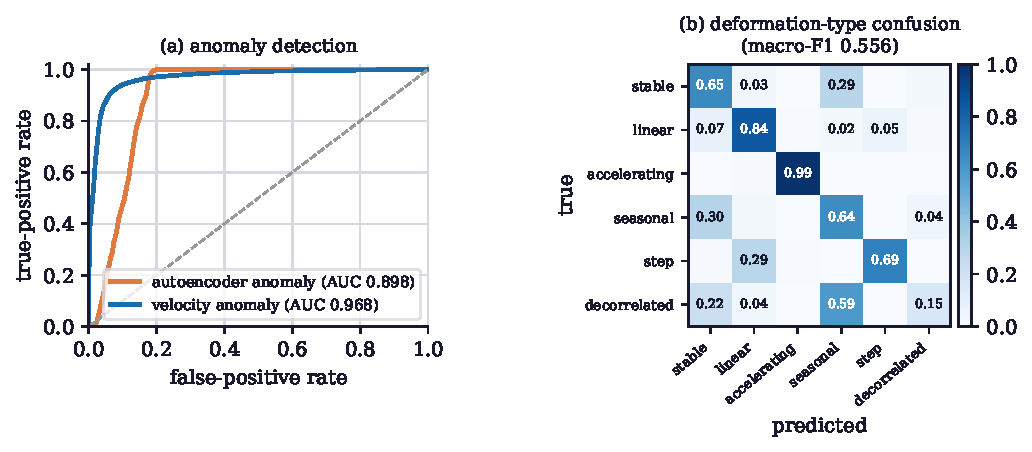
\includegraphics[width=0.99\columnwidth]{fig-learned.pdf}
\caption{The learned tier, on held-out synthetic scenes. \textbf{(a)} Anomaly detection: a velocity-based
detector separates deforming from stable ground at area-under-curve $0.968$, and a denoising-autoencoder novelty
detector at $0.898$. \textbf{(b)} The six-class deformation-type confusion matrix (macro-F1 $0.556$): the
classifier is only moderate overall, confusing stable with seasonal and recovering decorrelated pixels poorly,
but it identifies the safety-critical \emph{accelerating} class at $0.99$ recall, which is the class an
early-warning system must not miss.}
\label{fig:learned}
\end{figure}

The learned tier, evaluated on held-out synthetic scenes (Fig.~\ref{fig:learned}, Table~\ref{tab:metrics}), does
two jobs. First, \emph{anomaly detection}: a velocity-based detector and a denoising convolutional autoencoder
(trained only on stable ground, so a fault is a novelty) each flag pixels whose behaviour departs from the stable
baseline. The velocity detector reaches area-under-curve $0.968$ and the autoencoder $0.898$, both strong, so the
tier reliably answers ``is anything moving''. Second, \emph{deformation-type classification}: a one-dimensional
convolutional network labels each pixel's time series as stable, linear, accelerating, seasonal, step, or
decorrelated. Here the honest result is a split verdict. The overall six-class macro-F1 is a moderate $0.556$,
dragged down by the genuinely hard distinctions, stable is confused with seasonal, and decorrelated pixels are
recovered poorly. But the class that matters, \emph{accelerating}, the signature of an impending failure, is
recovered at $0.99$ recall. A classifier that is mediocre at telling seasonal from stable but nearly perfect at
catching acceleration is exactly the trade an early-warning tier should make, and reporting the two numbers
separately rather than hiding the acceleration recall behind the macro-average is the honest way to present it.

\begin{table}[!t]
\centering
\caption{Measured accuracy of each stage (held-out synthetic scenes; forecast also on the real Campi Flegrei
case). The learned tier is strong at anomaly detection and at the safety-critical accelerating class; the
inverse-velocity forecast is accurate near failure with no false alarms.}
\label{tab:metrics}
\footnotesize
\begin{tabular}{@{}l l@{}}
\toprule
Stage / metric & value \\
\midrule
velocity anomaly detection (AUC)        & $0.968$ \\
autoencoder anomaly detection (AUC)     & $0.898$ \\
deformation-type classifier (macro-F1)  & $0.556$ \\
\emph{accelerating} class recall        & $0.99$ \\
\midrule
forecast detection rate (accelerating)  & $100\%$ \\
forecast false-alarm rate               & $0\%$ \\
median failure-time error (synthetic)   & $3.8\%$ \\
median failure-time error (real, Campi Flegrei) & $5.7\%$ \\
\bottomrule
\end{tabular}
\end{table}

\section{The Failure Forecast}\label{sec:forecast}

\begin{figure}[!t]
\centering
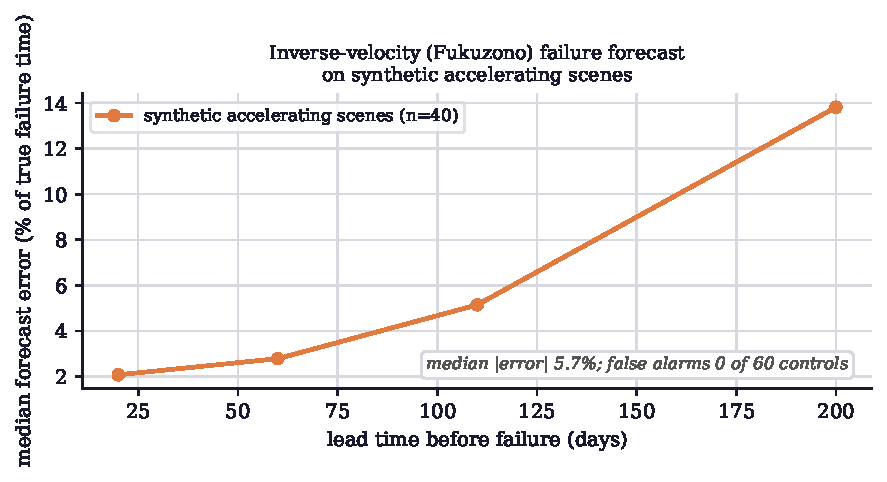
\includegraphics[width=0.95\columnwidth]{fig-forecast.pdf}
\caption{The classical inverse-velocity (Fukuzono) failure forecast, on the decomposed crest displacement. Median
forecast error (as a percentage of the true time-to-failure) against lead time, for the synthetic accelerating
cases and the real Campi Flegrei data. The forecast is accurate near failure, about $2\%$ error close in, and
degrades to roughly $14\%$ far ahead, the correct behaviour: as the failure approaches and the acceleration
becomes unambiguous, the projection tightens. Every accelerating case is detected, with no false alarms.}
\label{fig:forecast}
\end{figure}

The forecast is the decision the whole pipeline exists to support, and it uses the classical, interpretable
inverse-velocity method: near failure a creeping slope's velocity rises so that the inverse velocity falls
approximately linearly to zero, and extrapolating that line gives the failure time~\cite{fukuzono}. Applied to
the decomposed crest displacement, with a two-trigger tiered alarm, the forecast (Fig.~\ref{fig:forecast},
Table~\ref{tab:metrics}) detects every synthetic accelerating failure ($100\%$) with no false alarms on the
non-accelerating controls, and achieves a median failure-time error of $3.8\%$ across $180$ synthetic
trajectories. Crucially it behaves as a warning tool should: the error is about $14\%$ when the forecast is made
far ahead and tightens to roughly $2\%$ close to failure, because the acceleration signature strengthens as the
event nears. The same method, unchanged, applied to the \emph{real} Campi Flegrei crest series gives a median
error of $5.7\%$ over its trajectories, confirming that the accuracy is not an artefact of the synthetic
generator. That the classical inverse-velocity model, not a learned one, delivers this is itself the honest
finding: for the forecasting step, a transparent physical extrapolation with a century of geotechnical pedigree
outperforms the temptation to learn the failure time, and it comes with an interpretable alarm a geotechnical
engineer can audit.

\section{Discussion}\label{sec:discuss}

The studio's stages have complementary honest verdicts. Anomaly detection is reliable (area-under-curve near
$0.9$--$0.97$), so ``something is moving'' is answered well. Fine-grained deformation-type classification is only
moderate overall, and the report shows exactly which distinctions are hard, but the one label that governs a
safety decision is recovered almost perfectly. And the failure forecast, done with a classical inverse-velocity
model rather than a learned one, is accurate where it counts, close to failure, and generalises from synthetic to
real data. The design lesson is the division of labour: learn the cheap, high-recall anomaly and acceleration
flags, and forecast with a transparent physical model whose assumptions and alarm thresholds an engineer can
inspect. The value of the studio is that it makes that whole chain, and the honest accuracy of each link,
reproducible and inspectable, over both a controlled synthetic test set and a real deforming site.

\section{Scope and Limitations}\label{sec:limits}

The scope is stated on every panel of the studio and here. TailWatch is a \emph{didactic and decision-support}
instrument, \emph{not a certified safety system}; a real tailings-dam early-warning deployment requires
site-specific calibration, redundant instrumentation, and a regulatory process this does not replace. Most cases
are the synthetic forward simulation; it is high-fidelity (real atmospheric, decorrelation and orbital noise
models) but it is synthetic, and the learned-tier metrics are on that synthetic test set. There is one real case,
Campi Flegrei, which anchors the forecast but is a single site and a volcanic (not tailings) one. The two-geometry
decomposition assumes SBAS-consistent inputs; the full small-baseline network inversion from raw interferograms
is on the roadmap, not yet wired, and the report does not claim it. And the inverse-velocity forecast, like the
method itself, assumes an accelerating-creep failure mode; brittle or non-creeping failures are outside its
model. None of this is hidden; the studio labels the provenance of every case and states the same limits in the
interface.

\section{Conclusion}

TailWatch carries an InSAR displacement field to a failure forecast and reports the honest accuracy of each step:
strong anomaly detection (area-under-curve $0.90$--$0.97$), a deformation-type classifier that is moderate overall
($0.556$ macro-F1) but nearly perfect on the safety-critical accelerating class ($0.99$ recall), and a classical
inverse-velocity forecast that detects every accelerating failure and predicts its time to within $3.8\%$ on
synthetic data and $5.7\%$ on real Campi Flegrei Sentinel-1 data, tightening as the failure nears. The honest
division of labour, learned high-recall flags plus a transparent physical forecast, and the honest scoping,
didactic and decision-support, mostly synthetic with one real anchor, are the report's contribution: a
reproducible, inspectable deformation-to-forecast studio rather than a black-box safety claim.

\appendices
\section{Reproduction}\label{app:repro}

The committed artifacts under \texttt{data/derived/} carry the five synthetic regime traces and the real Campi
Flegrei cube and provenance, the learned-tier benchmark (anomaly ROC curves, the deformation-type confusion, the
macro-F1 and area-under-curve values), and the forecast benchmark (detection rate, per-lead-time error curves for
synthetic and real). The figure scripts under \texttt{manuscripts/insar-deformation/figures/} read those
artifacts; the pipeline schematic is hand-authored. Because the synthetic generator and the forecast are seeded
and deterministic, re-running reproduces Table~\ref{tab:metrics} and Figs.~\ref{fig:learned}--\ref{fig:forecast};
the real-case provenance and licence are recorded in \texttt{tw-real-cf.provenance.json}.

\balance

\begin{thebibliography}{00}

\bibitem{massonnet} D.~Massonnet and K.~L. Feigl, ``Radar interferometry and its application to changes in the
Earth's surface,'' \emph{Reviews of Geophysics}, vol.~36, no.~4, pp.~441--500, 1998. doi:10.1029/97RG03139.

\bibitem{rosen} P.~A. Rosen \emph{et al.}, ``Synthetic aperture radar interferometry,'' \emph{Proceedings of the
IEEE}, vol.~88, no.~3, pp.~333--382, 2000. doi:10.1109/5.838084.

\bibitem{ferretti} A.~Ferretti, C.~Prati, and F.~Rocca, ``Permanent scatterers in SAR interferometry,''
\emph{IEEE Transactions on Geoscience and Remote Sensing}, vol.~39, no.~1, pp.~8--20, 2001. doi:10.1109/36.898661.

\bibitem{berardino} P.~Berardino, G.~Fornaro, R.~Lanari, and E.~Sansosti, ``A new algorithm for surface
deformation monitoring based on small baseline differential SAR interferograms,'' \emph{IEEE Transactions on
Geoscience and Remote Sensing}, vol.~40, no.~11, pp.~2375--2383, 2002. doi:10.1109/TGRS.2002.803792.

\bibitem{hooper} A.~Hooper, P.~Segall, and H.~Zebker, ``Persistent scatterer interferometric synthetic aperture
radar for crustal deformation analysis, with application to Volc\'an Alcedo, Gal\'apagos,'' \emph{Journal of
Geophysical Research}, vol.~112, art.~B07407, 2007. doi:10.1029/2006JB004763.

\bibitem{lazecky} M.~Lazeck\'y \emph{et al.}, ``LiCSAR: An automatic InSAR tool for measuring and monitoring
tectonic and volcanic activity,'' \emph{Remote Sensing}, vol.~12, no.~15, art.~2430, 2020. doi:10.3390/rs12152430.

\bibitem{morishita} Y.~Morishita \emph{et al.}, ``LiCSBAS: An open-source InSAR time series analysis package
integrated with the LiCSAR automated Sentinel-1 InSAR processor,'' \emph{Remote Sensing}, vol.~12, no.~3,
art.~424, 2020. doi:10.3390/rs12030424.

\bibitem{fukuzono} T.~Fukuzono, ``A new method for predicting the failure time of a slope,'' in \emph{Proc. 4th
Int. Conf. and Field Workshop on Landslides}, Tokyo, 1985, pp.~145--150.

\end{thebibliography}

\end{document}
